% compact.tex — Andrea Zignoli — Short CV
% Compile with: lualatex compact.tex
\documentclass[10pt,a4paper]{article}

\usepackage{geometry}
\geometry{top=1.5cm, bottom=1.5cm, left=1.8cm, right=1.8cm}

\usepackage{fontspec}
\setmainfont{Ubuntu}

\usepackage[T1]{fontenc}
\usepackage{microtype}
\usepackage{parskip}
\setlength{\parskip}{3pt}
\setlength{\parindent}{0pt}
\usepackage{setspace}
\setstretch{1.1}

\usepackage{titlesec}
\titleformat{\section}{\normalsize\bfseries\uppercase}{}{0em}{}[\vspace{-4pt}\rule{\linewidth}{0.6pt}\vspace{2pt}]
\titlespacing{\section}{0pt}{12pt}{6pt}

\usepackage{enumitem}
\setlist[itemize]{itemsep=2pt, topsep=3pt, partopsep=0pt, leftmargin=1.4em}
\setlist[enumerate]{itemsep=2pt, topsep=3pt, partopsep=0pt, leftmargin=1.6em}

\usepackage{array, booktabs, tabularx}
\usepackage{multicol}
\usepackage{tikz}
\usepackage{xcolor}
\definecolor{linkcolor}{HTML}{1a1a8c}
\usepackage[colorlinks=true, urlcolor=linkcolor, hidelinks,
  pdftitle={Andrea Zignoli -- Curriculum Vitae},
  pdfauthor={Andrea Zignoli},
  pdfsubject={CV}]{hyperref}

% ── helper: right-aligned date on same line as role ──────────────────────────
\newcommand{\entry}[3]{%          {Date}{Role/Title}{Institution}
  \textbf{#2}\hfill\textit{\small#1}\\[1pt]
  \small#3\par\vspace{5pt}%
}
\newcommand{\pub}[3]{%            {Authors}{Title}{Venue, Year}
  \hangindent=1em\hangafter=1
  \small #1. \textit{#2}. #3.\par\vspace{3pt}%
}

\pagestyle{plain}

\begin{document}

%% ── HEADER ─────────────────────────────────────────────────────────────────
\begin{center}
  \begin{tikzpicture}
    \clip (0,0) circle (1.1cm);
    \node at (0,0) {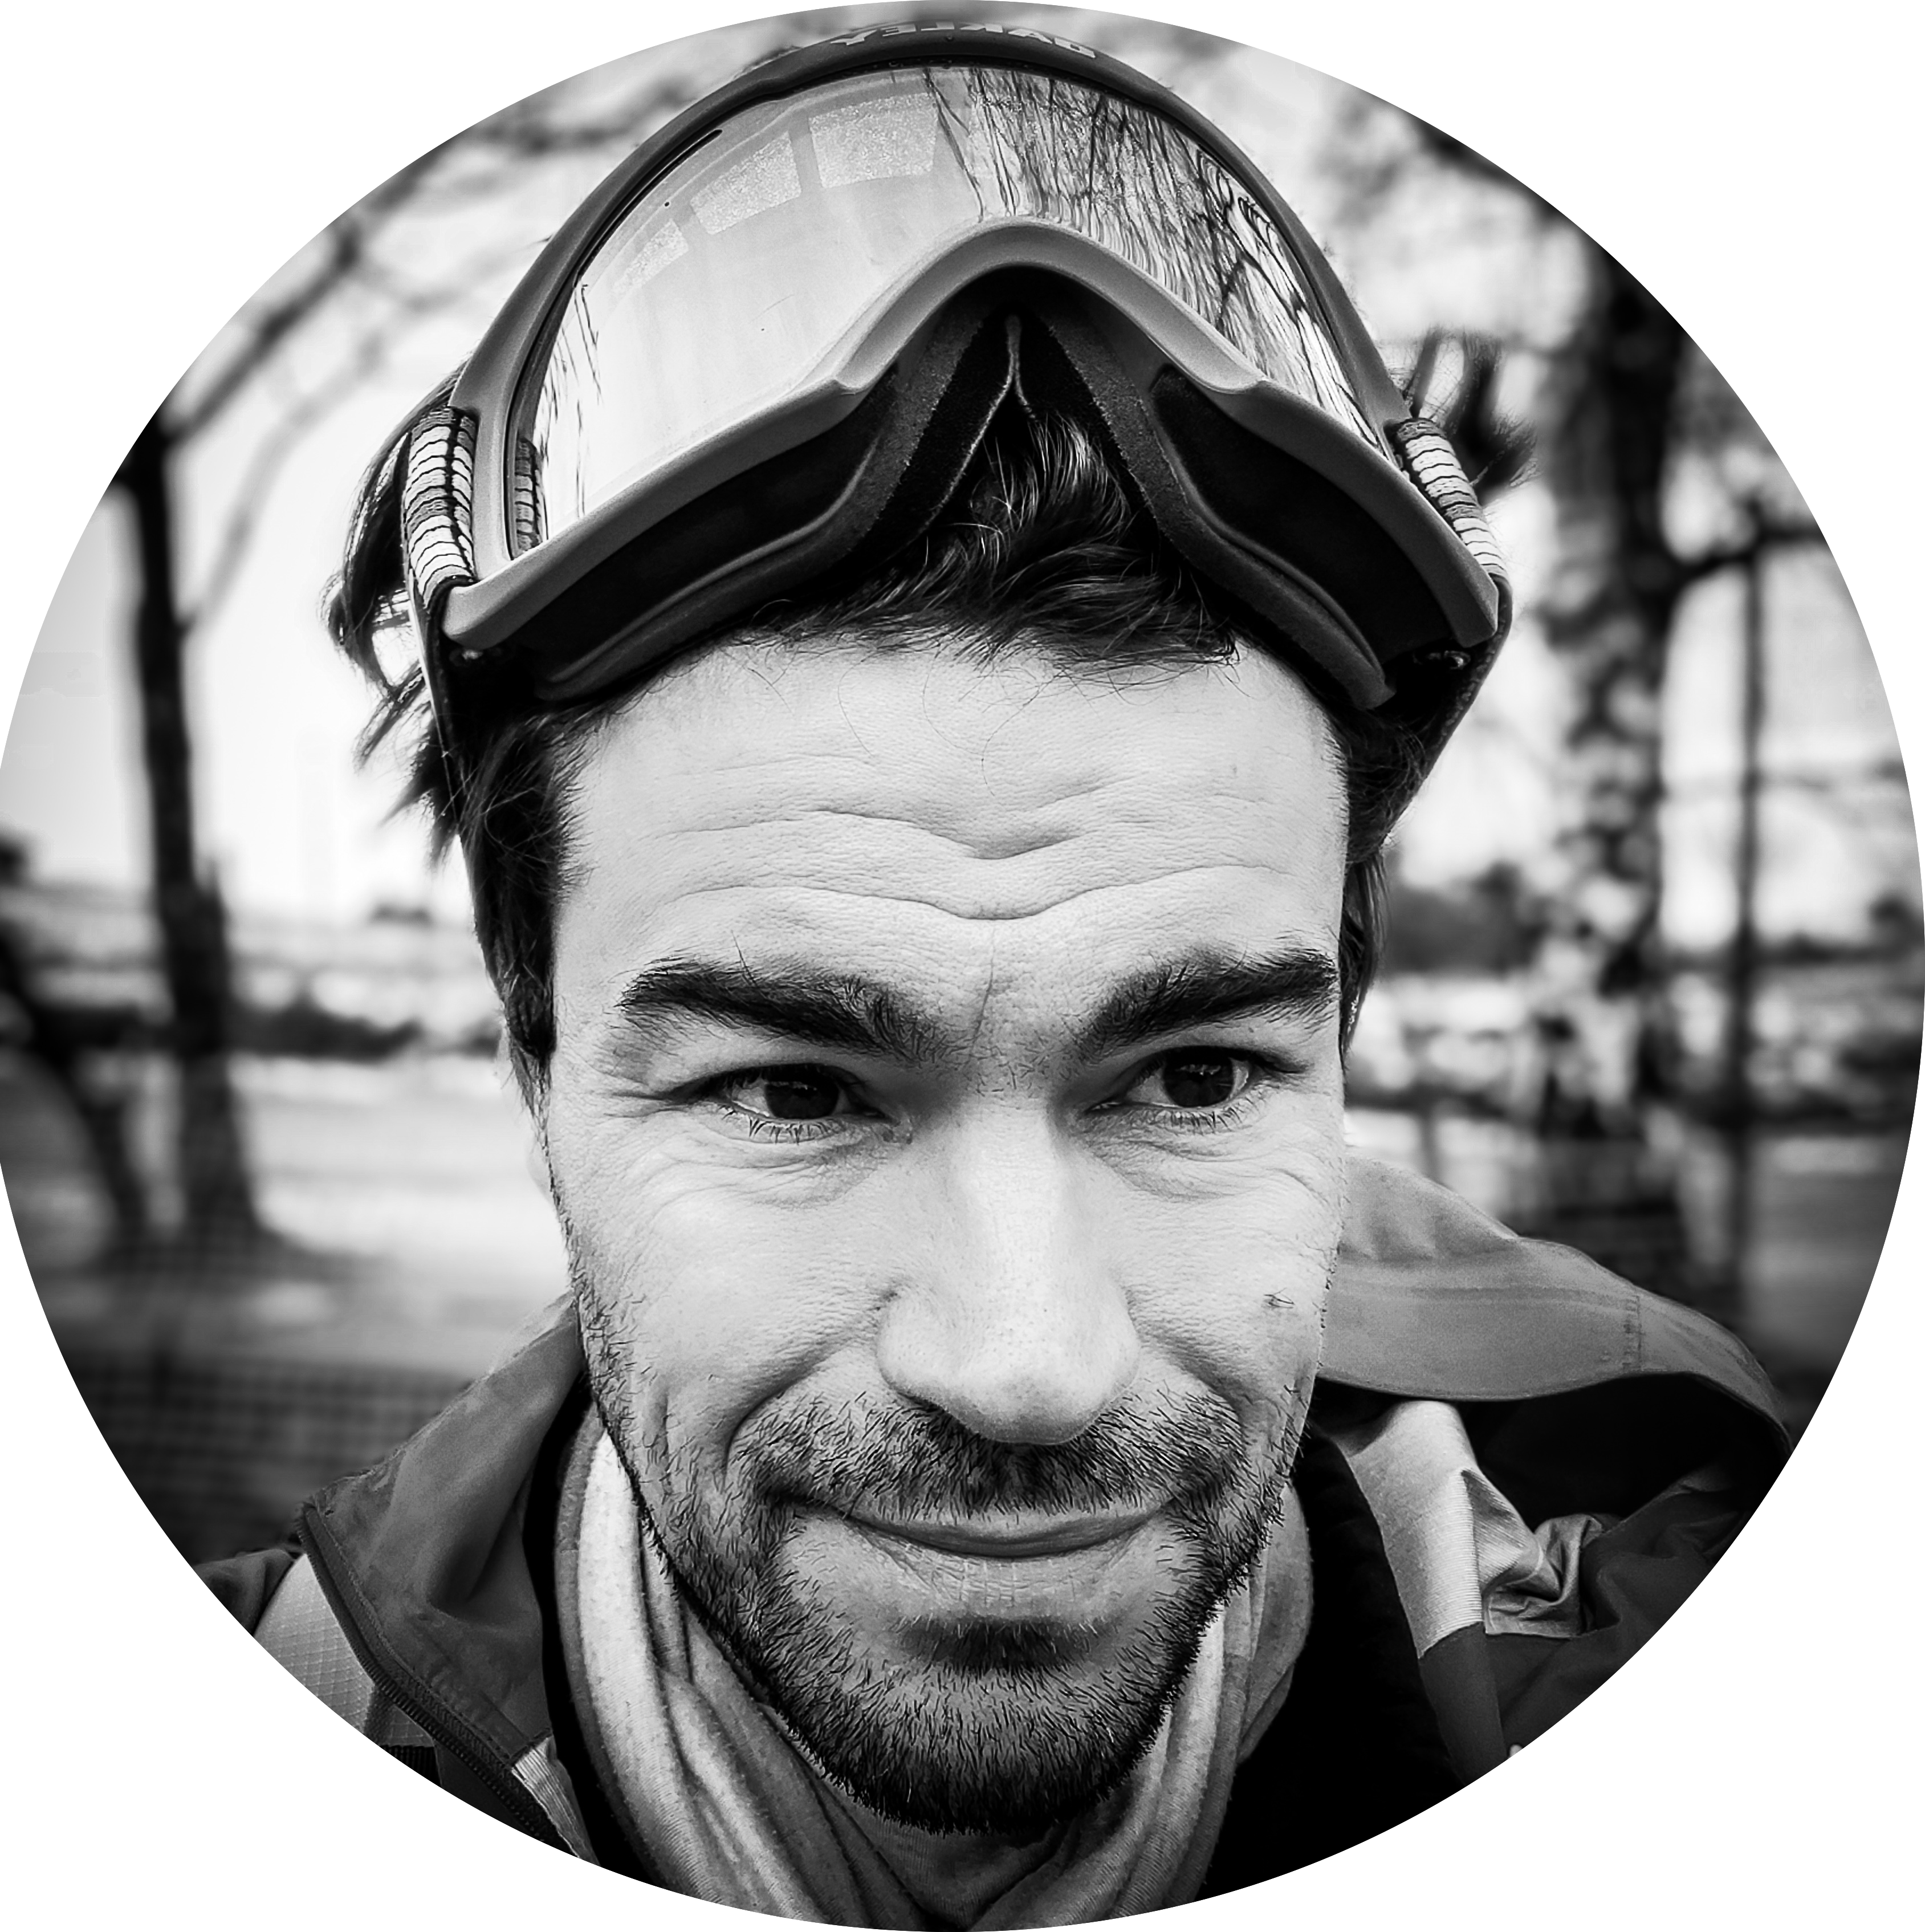
\includegraphics[width=2.2cm]{profile_pic_1_1.png}};
  \end{tikzpicture}\\[6pt]
  {\LARGE\bfseries Andrea Zignoli}\\[4pt]
  {\small
    San Pietro In Cariano, Italy \quad|\quad
    \href{mailto:andrea.zignoli@unitn.it}{andrea.zignoli@unitn.it} \quad|\quad
    \href{https://andreazignoli.com}{andreazignoli.com} \quad|\quad
    \href{https://andreazignoli.github.io}{andreazignoli.github.io} \quad|\quad
    \href{https://linkedin.com/in/andrea-zignoli-8080a438}{LinkedIn} \quad|\quad
    \href{https://github.com/andreazignoli}{GitHub}
  }
\end{center}
\vspace{4pt}

{\small Applied research scientist with 10+ years of experience developing AI-driven solutions for health and sports performance analysis. Specializes in deep learning on physiological signals, rigorous statistical evaluation, and model robustness under real-world distributional shifts. M.Eng.\ (Mechatronics) and PhD (Movement Science). Associate Editor, Sports Engineering (Springer).}

%% ── CURRENT POSITIONS ───────────────────────────────────────────────────────
\section{Current Positions}

\entry{Jan 2025 – present}{AI Consultant — Enhance-d}{Sports nutrition platform: agentic AI frameworks, LLM pipelines, and backend systems for personalized nutrition.}
\entry{Dec 2024 – present}{AI Consultant — Tyme Wear}{Wearable health tech: deep learning models for physiological signal processing and backend solutions.}
\entry{Apr 2020 – present}{Applied Research Scientist / Product Expert — Athletica Inc.}{Back-end lead: data processing \& analysis for a web-based endurance training platform.}
\entry{Dec 2021 – present}{Teaching Fellow — CIBIO, University of Trento}{3-credit module on Modelling, MSc Exercise Science and Human Movement.}
\entry{Apr 2022 – present}{Fellow Researcher — Dept.\ Industrial Engineering, University of Trento}{Mathematical models for sport technology applications.}
\entry{Dec 2021 – present}{Associate Editor — Sports Engineering Journal (Springer)}{Manuscript handling; partnerships with sport-tech companies and governing bodies.}

%% ── WORK \& RESEARCH EXPERIENCE ────────────────────────────────────────────
\section{Work \& Research Experience}

\entry{Apr 2021 – Mar 2024}{Full-time Data Scientist — Supersapiens}{CGM signal processing, time-series analysis, anomaly detection, pattern recognition.}
\entry{Apr 2022 – Nov 2022}{Visiting Researcher — University of Queensland, Brisbane, AU}{School of Human Movement and Nutrition Sciences. Ref: Jeff Coombes.}
\entry{Oct 2021 – Apr 2022}{Visiting Researcher — University of Southern Denmark, Odense, DK}{Muscle Physiology and Biomechanics; Center for Active and Healthy Aging. Ref: Paolo Caserotti.}
\entry{Dec 2020 – Dec 2021}{Postdoctoral Researcher — University of Trento}{First-principle and data-driven models for sport tech; TRL 3–4 prototypes. Ref: F.\ Biral.}
\entry{Nov 2019 – Nov 2020}{Postdoctoral Researcher — University of Trento (DDL-Meccatronica)}{Setup of Deep Learning Lab at ProM Facility, Trento. Ref: P.\ Bosetti.}
\entry{Nov 2017 – Nov 2019}{Postdoctoral Researcher — University of Trento (\textit{De Motu})}{Kinematic modelling of the human knee; partners: ProM, CeRiSM, MUSE. Ref: F.\ Biral.}
\entry{Nov 2016 – May 2017}{Visiting Researcher — KAST, Kawasaki, JP}{Haptic robots for medicine, rehabilitation and welfare. Ref: T.\ Shimono.}
\entry{Jan 2013 – Dec 2015}{PhD Student — CeRiSM / University of Verona}{Bioenergetic \& biomechanical models of cycling; optimal control. Tutors: B.\ Pellegrini \& F.\ Biral.}
\entry{Mar – Sept 2015}{Visiting PhD Student — Human Performance Lab, University of Calgary, CA}{Musculoskeletal modelling of the human lower limb. Ref: W.\ Herzog.}
\entry{Sept 2010 – Mar 2011}{Visiting Master Student — University of Nottingham, UK}{Mathematical models of driver behaviour. Ref: A.A.\ Popov.}

%% ── EDUCATION ───────────────────────────────────────────────────────────────
\section{Education}

\entry{2013 – 2016}{PhD — Movement Science \& Physical Exercise, University of Verona}{\textit{Development of integrated tools for bio-mechanical analysis in sport performance: application to cycling.} Tutors: B.\ Pellegrini \& F.\ Biral.}
\entry{2008 – 2011}{M.Eng.\ Mechatronics (105/110) — University of Trento}{\textit{Applications of Control Techniques to the Modeling of Driver Behavior.} Advisors: F.\ Biral \& A.A.\ Popov.}
\entry{2003 – 2008}{B.Eng.\ Industrial Engineering (92/110) — University of Trento}{\textit{Individuazione Statistica dell'Interfaccia di Cavitazione.} Advisor: F.\ Trivellato.}

%% ── SKILLS ──────────────────────────────────────────────────────────────────
\section{Technical Skills}

\begin{multicols}{2}
\textbf{Languages:} Python (10+ yrs), Matlab, R, \LaTeX, C/C++\\
\textbf{ML/DL:} scikit-learn, TensorFlow/Keras, LSTM, CNN, GAN; familiar with self-supervised learning \& parameter-efficient fine-tuning (LoRA)\\
\textbf{LLM/Agents:} RAG pipelines, agentic frameworks, Claude Code\\
\textbf{Signal processing:} EMG, CPET, GPS, IMU, CGM, power meters\\
\textbf{Stats:} hypothesis testing, uncertainty quantification, ANOVA, RM-ANOVA, multi-linear models, PCA, longitudinal analysis\\
\textbf{Backend/DevOps:} FastAPI, Flask, Docker, AWS Lambda, Heroku\\
\textbf{Optimal control:} GPOPS-II, PINS, first-principles modelling
\end{multicols}

%% ── FUNDINGS ────────────────────────────────────────────────────────────────
\section{Funding \& Grants (selected)}

\begin{itemize}
  \item ANTA Award (ECSS) — \textit{DARDAR project}: stride-by-stride running kinematics in real-life conditions (w/ Univ.\ Franche Comté). €20{,}000.
  \item ATHLETICA project: web-based training data platform. €9{,}600.
  \item Selle Royal: testing protocol for high-level cycling shoes. €15{,}000.
  \item CARITRO DDL-Meccatronica post-doctoral fellowship (Deep Learning Lab, ProM). €35{,}000.
  \item CARITRO \textit{De Motu} post-doctoral fellowship (Dept.\ Industrial Engineering, Trento). €25{,}000.
  \item Starting Grant Young Researchers 2018, Univ.\ Trento (w/ Prof.\ M.\ Pandy, Univ.\ Melbourne). €5{,}000.
  \item International Cooperation Grant 2015 — \textit{Modeling the Lower Limb of Cyclist}, Calgary. €3{,}000.
  \item PhD scholarship, University of Verona (2013–2015). €60{,}000.
  \item Erasmus scholarship, Univ.\ Nottingham (2010–2011). €3{,}000.
\end{itemize}

%% ── PUBLICATIONS ────────────────────────────────────────────────────────────
\section{Publications — Journal Papers (Leading Author, newest first)}

\pub{D. Keir, \textbf{A. Zignoli}, F.M. Maturana, D. Iannetta, J.M. Murias}{AI-driven analysis of cardiopulmonary exercise tests to identify gas exchange and ventilatory thresholds}{Sports Medicine, 2026}

\pub{\textbf{A. Zignoli}}{Assessing trajectories and bike handling abilities in road cycling with global positioning system data}{Sensors, 2025}

\pub{\textbf{A. Zignoli}, P. Whitehurst}{Real-time assessment of exercising maximal mean power and speed in endurance sports: a Garmin Connect IQ App}{Sports Engineering (Technical Note), 2025}

\pub{\textbf{A. Zignoli}, B. Martinez-Gonzalez, K. Skroce, D.J. Lipman, H.C. Zisser, A. Giorgi}{Personalized nutrition and machine-learning: exploring the scope of continuous glucose monitoring in healthy individuals in uncontrolled settings}{Int J Sport Nutr Exerc Metab., 2024}

\pub{\textbf{A. Zignoli}, K. Skroce, D.J. Lipman, H.C. Zisser}{Personalized nutrition and machine-learning: exploring the scope of CGM in healthy individuals}{Biomedical Signal Processing and Control, 2023}

\pub{\textbf{A. Zignoli}, A. Godin, L. Mourot}{Indoor running temporal variability for different speeds, inclinations, and estimation strategies}{PLOS ONE, 2023}

\pub{\textbf{A. Zignoli}, F.Y. Fontana, K. Skroce, D.J. Lipman, F.M. Maturana, H.C. Zisser}{Association between pre-exercise food ingestion timing and reactive hypoglycemia}{European Journal of Sport Science, 2023}

\pub{\textbf{A. Zignoli}, A. Fornasiero, F. Gilli, B. Pellegrini, F. Schena}{How the Oxynet web applications are used to crowdsource and interpret CPET data}{Biomedical Signal Processing and Control, 2023}

\pub{\textbf{A. Zignoli}}{Machine learning models for automatic detection of exercise thresholds in CPETs: from regression to generation to explanation}{Sensors, 2023}

\pub{\textbf{A. Zignoli}, D. Fruet}{Insights in road cycling downhill performance using aerial drone footages and an `optimal' reference trajectory}{Sports Engineering (Technical Note), 2022}

\pub{\textbf{A. Zignoli}}{An intelligent curve warning system for road cycling races}{Sports Engineering (Technical Note), 2021}

\pub{\textbf{A. Zignoli}, F. Biral, A. Fornasiero, D. Sanders, T. Van Erp, M. Mateo-March \textit{et al.}}{Assessment of bike handling during cycling individual time trials with a novel analytical technique}{European Journal of Sport Science, 2021}

\pub{\textbf{A. Zignoli}, A. Fornasiero, P. Rota, V. Muollo, L.A. Peyré-Tartaruga, D.A. Low \textit{et al.}}{Oxynet: a collective intelligence that detects ventilatory thresholds in cardiopulmonary exercise tests — crowdsourced across heterogeneous labs, devices, and operators to characterise model robustness under real-world distributional shifts}{European Journal of Sport Science, 2020}

\pub{\textbf{A. Zignoli}}{Influence of corners and road conditions on cycling individual time trial performance and optimal pacing strategy}{Journal of Sports Engineering and Technology, 2020}

\pub{\textbf{A. Zignoli}, A. Fornasiero, M. Ragni, B. Pellegrini, F. Schena, F. Biral, P.B. Laursen}{Estimating an individual's oxygen consumption during cycling with a recurrent neural network}{PLOS ONE, 2020}

\pub{\textbf{A. Zignoli}, F. Biral}{A new optimal control framework to predict realistic pacing and cornering strategies during cycling individual time trials}{Sports Engineering, 2020}

\pub{\textbf{A. Zignoli}, A. Fornasiero, E. Bertolazzi, B. Pellegrini, F. Schena, F. Biral, P.B. Laursen}{State-of-the-art concepts and future directions in modelling oxygen consumption and lactate concentration in cycling}{Sport Science for Health, 2019}

\pub{\textbf{A. Zignoli}, A. Fornasiero, F. Stella, B. Pellegrini, F. Schena, F. Biral, P.B. Laursen}{Expert-level classification of ventilatory thresholds from CPET data with recurrent neural networks}{European Journal of Sport Science, 2019}

\pub{\textbf{A. Zignoli}, F. Biral, B. Pellegrini, A. Jinha, W. Herzog, F. Schena}{Optimal control solution to the predictive dynamics of cycling}{Sport Science for Health, 2017}

\section{Publications — Journal Papers (Co-Author, newest first)}

\pub{B. Bizet, M. Trinchi, F. Nardello, F. Bombieri, \textbf{A. Zignoli}, P. Zamparo, A. Monte}{Quantitative ultrasound radiofrequency analysis for monitoring Parkinson's disease}{Neuroscience, 2026}

\pub{K. Skroce, L.V. Turner, \textbf{A. Zignoli}, D.J. Lipman, H.C. Zisser, M.C. Riddell}{Beyond Euglycemia: Case Studies Using CGM in Elite Athletes Without Diabetes During Record Events}{(in press)}

\pub{K. Skroce, \textbf{A. Zignoli}, L.V. Turner, D.J. Lipman, M.C. Riddell, H.C. Zisser}{CGM-derived glucose metrics over time in physically active adults without diabetes}{(in press)}

\pub{F. Malizia, \textbf{A. Zignoli}, K.E. Teigen Giljarhus}{Topical collection: Fluid Dynamics in Sports}{Sports Engineering, 2025}

\pub{K. Skroce, \textbf{A. Zignoli}, N. Mihic, D.J. Lipman, L.V. Turner, M.C. Riddell, H.C. Zisser}{Continuous Glucose Monitoring Profiles in Elite-Level Professional European Football Players}{Journal of Diabetes Science and Technology, 2025}

\pub{A. Fornasiero, A.G. Represas, \textbf{A. Zignoli}, F. Stella, M. Rakobowchuk, L. Mourot}{Moderate heart rate-matched hypoxic exercise: autonomic and cardiovascular responses}{European Journal of Applied Physiology, 2025}

\pub{M. Tarocchi, A. Pellegrino, K. Skroce, \textbf{A. Zignoli} \textit{et al.}}{Assessing Energy Availability and Glucose Dynamics in Adolescent Cyclists}{Nutrients, 2024}

\pub{D. Fruet, \textbf{A. Zignoli}, R. Modena, B. Pellegrini, L. Gastaldi, L. Bortolan}{Design and development of a feedback system for automatic treadmill speed adaptation}{Proc.\ IMechE Part P: J.\ Sports Eng.\ Tech., 2024}

\pub{K. Skroce, \textbf{A. Zignoli}, F.Y. Fontana, F.M. Maturana, D. Lipman, A. Tryfonos, M.C. Riddell, H.C. Zisser}{Real World Interstitial Glucose Profiles of a Large Cohort of Physically Active Men and Women}{Sensors, 2024}

\pub{A. Fornasiero, \textbf{A. Zignoli}, B. Pellegrini, F. Schena, G. Doucende, L. Mourot}{Effects of a 6-hour ultra-endurance run on post-exercise parasympathetic reactivation responses}{J.\ Sports Medicine and Physical Fitness, 2023}

\pub{A. Fornasiero, A. Savoldelli, \textbf{A. Zignoli} \textit{et al.}}{Eager to set a record in a vertical race? Test your VO2max first!}{Journal of Sports Sciences, 2023}

\pub{V. Muollo, \textbf{A. Zignoli}, L. Ghiotto \textit{et al.}}{Knee flexor and extensor torque ratio in elderly men and women with and without obesity}{Aging Clinical and Experimental Research, 2021}

\pub{A. Fornasiero, \textbf{A. Zignoli}, M. Rakobowchuk \textit{et al.}}{Post-exercise cardiac autonomic and cardiovascular responses to HR-matched and work rate-matched hypoxic exercise}{European Journal of Applied Physiology, 2021}

\pub{V. Muollo, A. Rossi, \textbf{A. Zignoli} \textit{et al.}}{Full characterisation of knee extensors' function in ageing: effect of sex and obesity}{International Journal of Obesity, 2020}

\pub{A. Monte, \textbf{A. Zignoli}}{Muscle and tendon stiffness and belly gearing positively correlate with rate of torque development}{Journal of Biomechanics, 2020}

\pub{L. Mourot, A. Fornasiero, M. Rakobowchuk, \textbf{A. Zignoli} \textit{et al.}}{Post-exercise hypotension and reduced cardiac baroreflex after half-marathon run: in men, not in women}{Int.\ J.\ Environmental Research and Public Health, 2020}

\pub{A. Fornasiero, A. Savoldelli, \textbf{A. Zignoli} \textit{et al.}}{Shortening Work-Rest Durations Reduces Physiological and Perceptual Load During Uphill Walking in Cold High-Altitude Conditions}{High Altitude Medicine \& Biology, 2020}

\pub{L. Mourot, A. Fornasiero, \textbf{A. Zignoli} \textit{et al.}}{Similar cardiovascular and autonomic responses in trained T1DM and healthy participants after half marathon}{Diabetes Research and Clinical Practice, 2019}

\pub{A. Fornasiero, S. Skafidas, F. Stella, \textbf{A. Zignoli} \textit{et al.}}{Cardiac autonomic and physiological responses to moderate-intensity exercise in hypoxia}{Int.\ Journal of Sport Medicine, 2019}

\pub{A. Fornasiero, A. Savoldelli, \textbf{A. Zignoli} \textit{et al.}}{Delayed parasympathetic reactivation and sympathetic withdrawal following maximal CPET in hypoxia}{European Journal of Applied Physiology, 2018}

\pub{A. Fornasiero, A. Savoldelli, G. Boccia, \textbf{A. Zignoli} \textit{et al.}}{Physiological factors associated with ski-mountaineering vertical race performance}{Sport Science for Health, 2017}

\pub{G. Vernillo, A. Savoldelli, \textbf{A. Zignoli} \textit{et al.}}{An Extreme Mountain Ultra-Marathon Decreases the Cost of Uphill Walking and Running}{Frontiers in Physiology, 2016}

\pub{G. Vernillo, A. Savoldelli, \textbf{A. Zignoli} \textit{et al.}}{Energy Cost and Kinematics of Level, Uphill and Downhill Running: Fatigue-Induced Changes After a Mountain Ultramarathon}{Journal of Sports Science, 2015}

\pub{G. Vernillo, A. Savoldelli, \textbf{A. Zignoli} \textit{et al.}}{Influence of the world's most challenging mountain ultra-marathon on energy cost and running mechanics}{European Journal of Applied Physiology, 2014}

\section{Publications — Peer-Reviewed Conference Proceedings (newest first)}

\pub{A. Giorgi, B. Martinez-Gonzalez, M. Vicini, \textbf{A. Zignoli}, K. Skroce}{Continuous Glucose Monitoring of Non-Diabetic Professional Cyclists during a Training Camp}{Science \& Cycling Conf., 2023}

\pub{\textbf{A. Zignoli}, D. Fruet}{Automatic Generation of Realistic CPET Data With a Conditional Generative Adversarial Neural Network}{Workshop Sport, Technology and Research — IEEE, 2022}

\pub{D. Fruet, \textbf{A. Zignoli}, V. Fontanari \textit{et al.}}{Developing a Testing Protocol to Assess the Mechanical Properties of High-Level Cycling Shoes}{Workshop Sport, Technology and Research — IEEE, 2022}

\pub{\textbf{A. Zignoli}, L. Mourot, D. Fruet}{Estimating Running Kinematics Variability With an IMU Sensor on the Runner's Thorax}{Workshop Sport, Technology and Research — IEEE, 2022}

\pub{\textbf{A. Zignoli}, L. Tonelli, D. Fruet, F. Biral, V. Fontanari}{Biomechanical Analysis and Modeling of ACL Rupture Conditions: Focus on Female Soccer Players}{Workshop Sport, Technology and Research — IEEE, 2022}

\pub{N. Peghini, \textbf{A. Zignoli}, D. Gandolfi, P. Rota, P. Bosetti}{Real-time cross-dataset quality production assessment in industrial laser cutting machines}{1st Workshop Industrial Machine Learning — ICPR, 2020}

\pub{\textbf{A. Zignoli}, F. Biral, K. Yokoyama, T. Shimono}{Including a musculoskeletal model in the control loop of an assistive robot for optimal target forces}{IECON — IEEE Industrial Electronics Society, 2019}

\pub{\textbf{A. Zignoli}, T. Shimono, F. Biral}{Rationale for researching in DOB/OC-based rehabilitation robots: simulation results}{IECON — IEEE Industrial Electronics Society, 2018}

\pub{\textbf{A. Zignoli}, L. Beatrici, F. Biral}{Analysis of assistive strategies for electric bikes including rider physiological characteristics}{IDETC/CIE — ASME, 2018}

\pub{D. Fruet, \textbf{A. Zignoli}, L. Bortolan, L. Gastaldi, B. Pellegrini}{Kinect-based system for self-adjusting treadmill speed in cross-country indoor ski}{Int.\ Conf.\ Soft-Computing \& Networks, 2015}

\pub{\textbf{A. Zignoli}, F. Biral, A.A. Popov}{Application of non-linear model predictive control to the driving task}{FAST-zero Symposium, 2011}

\section{Conference Contributions (Selected, as Leading Author)}

\begin{itemize}
  \item \textit{Incorporating the maximal mean power profile in time trial simulations} — Cycling Science Conf., Florence, 2024.
  \item \textit{DeMotu project: design and production of a 3D printed human knee for biomechanics research} — MSH, 2019; ESB, 2019.
  \item \textit{Modeling the acute physiological response to cycling: the blood lactate concentration challenge} — Modelling in Endurance Sports Workshop, 2016.
  \item \textit{An optimal control approach to the HIIT design} — World Congress of Cycling Science, 2016.
  \item \textit{Application to cycling of a bioenergetic model} — World Congress of Cycling Science, 2014; MSH, 2013, 2015.
\end{itemize}

%% ── TEACHING \& SERVICE ─────────────────────────────────────────────────────
\section{Teaching, Mentoring \& Service}

\textbf{Teaching:}
\begin{itemize}
  \item 2019–2024: Lab module, \textit{Technology and Innovation in Sports}, MSc Phys.\ Ed., Univ.\ Verona / Trento.
  \item 2015–2018: Lab module, \textit{Technology of Measurement Systems}, MSc Phys.\ Ed., Univ.\ Verona.
  \item 2013–2015: Lab module, \textit{Movement and Sport Biomechanics}, MSc Phys.\ Ed., Univ.\ Verona.
\end{itemize}

\textbf{Co-advisor:} 9 master theses (Univ.\ Trento: Mechatronics, Materials Engineering; Univ.\ Verona: Phys.\ Ed.).

\textbf{Reviewer:} IECON, Transactions in Mechatronics, J.\ Sports Sciences, Frontiers in Physiology, Cycling Science Journal, SJMSS, Plos One, Sports Engineering, Nature Scientific Communications, and others.

%% ── MEDIA & OUTREACH ────────────────────────────────────────────────────────
\section{Media \& Outreach (Selected Podcast Appearances)}

\begin{itemize}
  \item \textit{AI Agents, HRV Readiness \& the Next Era of Training} — Training Science Podcast, Dec 2025.
  \item \textit{Modelling First: Building Smarter Endurance Training} — Training Science Podcast (Ep.\ 157), Mar 2025.
  \item \textit{Human-AI Balance in Coaching: AI-Assisted HRV Monitoring} — Athletes Compass Podcast, Dec 2024.
  \item \textit{From Lab to Athlete: Optimizing Training with Workout Reserve} — Athletes Compass Podcast, Oct 2024.
  \item \textit{What AI-Powered Training Is \& What It Is Not} — Paul Laursen Podcast, Jun 2022.
\end{itemize}

%% ── REFERENCES ──────────────────────────────────────────────────────────────
\section{References}

\textbf{Prof.\ Francesco Biral} — \href{mailto:francesco.biral@unitn.it}{francesco.biral@unitn.it} \quad
\textbf{Paul Laursen} — \href{mailto:paul@athletica.ai}{paul@athletica.ai}

\end{document}
